\documentclass[floatsintext,doc]{apa6}
\usepackage{lmodern}
\usepackage{amssymb,amsmath}
\usepackage{ifxetex,ifluatex}
\usepackage{apacite}
%\usepackage{hyperref}
\usepackage[utf8]{inputenc}
%\usepackage{fourier}%
%\usepackage{fourier}%
%\usepackage{heuristica}
\usepackage{geometry}

\usepackage{array}
\usepackage{tabularx}
\usepackage{caption}

\usepackage{fixltx2e} % provides \textsubscript
\ifnum 0\ifxetex 1\fi\ifluatex 1\fi=0 % if pdftex
  \usepackage[T1]{fontenc}
  \usepackage[utf8]{inputenc}
\else % if luatex or xelatex
  \ifxetex
    \usepackage{mathspec}
  \else
    \usepackage{fontspec}
  \fi
  \defaultfontfeatures{Ligatures=TeX,Scale=MatchLowercase}
\fi
% use upquote if available, for straight quotes in verbatim environments
\IfFileExists{upquote.sty}{\usepackage{upquote}}{}
% use microtype if available
\IfFileExists{microtype.sty}{%
\usepackage{microtype}
\UseMicrotypeSet[protrusion]{basicmath} % disable protrusion for tt fonts
}{}

%\hypersetup{unicode=true,
%            pdftitle={Not unreasonable: Uncertainty in the language of logic},
%            pdfauthor={Michael Henry Tessler~\& Michael Franke},
%            pdfkeywords={semantics; pragmatics; negation; Bayesian cognitive model; Rational Speech Act},
%            pdfborder={0 0 0},
%            breaklinks=true}
%\urlstyle{same}  % don't use monospace font for urls
\usepackage{graphicx,grffile}
\makeatletter
\def\maxwidth{\ifdim\Gin@nat@width>\linewidth\linewidth\else\Gin@nat@width\fi}
\def\maxheight{\ifdim\Gin@nat@height>\textheight\textheight\else\Gin@nat@height\fi}
\makeatother
% Scale images if necessary, so that they will not overflow the page
% margins by default, and it is still possible to overwrite the defaults
% using explicit options in \includegraphics[width, height, ...]{}
\setkeys{Gin}{width=\maxwidth,height=\maxheight,keepaspectratio}
\IfFileExists{parskip.sty}{%
\usepackage{parskip}
}{% else
\setlength{\parindent}{0pt}
\setlength{\parskip}{6pt plus 2pt minus 1pt}
}
\setlength{\emergencystretch}{3em}  % prevent overfull lines
\providecommand{\tightlist}{%
  \setlength{\itemsep}{0pt}\setlength{\parskip}{0pt}}
\setcounter{secnumdepth}{0}
% Redefines (sub)paragraphs to behave more like sections
\ifx\paragraph\undefined\else
\let\oldparagraph\paragraph
\renewcommand{\paragraph}[1]{\oldparagraph{#1}\mbox{}}
\fi
\ifx\subparagraph\undefined\else
\let\oldsubparagraph\subparagraph
\renewcommand{\subparagraph}[1]{\oldsubparagraph{#1}\mbox{}}
\fi

%%% Use protect on footnotes to avoid problems with footnotes in titles
\let\rmarkdownfootnote\footnote%
\def\footnote{\protect\rmarkdownfootnote}


%  \title{Not unreasonable: Uncertainty in the language of negation}
%  \title{Not unreasonable: Multiple opposite meanings are entertained when understanding negation}
%\title{Not stating the opposite: Double negations result in nonredundant meanings}
\title{Two negatives don't exactly make a positive}
    \author{Michael Henry Tessler\textsuperscript{1}~\& Michael Franke\textsuperscript{2}}
    \date{}
  
\shorttitle{Uncertain logical language}
\affiliation{
\vspace{0.5cm}
\textsuperscript{1} Massachusetts Institute of Technology\\\textsuperscript{2} University of Osnabr\"{u}ck}
\keywords{semantics; pragmatics; negation; Bayesian cognitive model; Rational Speech Act\newline\indent Word count: X}
\usepackage{csquotes}
\usepackage{upgreek}
\captionsetup{font=singlespacing,justification=justified}

\usepackage{longtable}
\usepackage{lscape}
\usepackage{multirow}
\usepackage{tabularx}
\usepackage[flushleft]{threeparttable}
\usepackage{threeparttablex}

%\newenvironment{lltable}{\begin{landscape}\begin{center}\begin{ThreePartTable}}{\end{ThreePartTable}\end{center}\end{landscape}}

\makeatletter
\newcommand\LastLTentrywidth{1em}
\newlength\longtablewidth
\setlength{\longtablewidth}{1in}
\newcommand{\getlongtablewidth}{\begingroup \ifcsname LT@\roman{LT@tables}\endcsname \global\longtablewidth=0pt \renewcommand{\LT@entry}[2]{\global\advance\longtablewidth by ##2\relax\gdef\LastLTentrywidth{##2}}\@nameuse{LT@\roman{LT@tables}} \fi \endgroup}


%\DeclareDelayedFloatFlavor{ThreePartTable}{table}
%\DeclareDelayedFloatFlavor{lltable}{table}
%\DeclareDelayedFloatFlavor*{longtable}{table}
\makeatletter
%\renewcommand{\efloat@iwrite}[1]{\immediate\expandafter\protected@write\csname efloat@post#1\endcsname{}}
\makeatother
\usepackage{tabularx}
\usepackage{multicol}
\usepackage{wrapfig}
\usepackage{gensymb}
\usepackage{tikz}
\usepackage{caption}
\usepackage{booktabs}
\usepackage{xcolor}

\authornote{This work was supported in part by NSF Graduate Research Fellowship DGE-114747 to MHT.

Correspondence concerning this article should be addressed to Michael Henry Tessler, 43 Vassar St, Cambridge, MA 02139. E-mail: \url{tessler@mit.edu}}

\abstract{
Logic tells us that two negatives make a positive, but in natural language, things are not so black and white: A person \emph{not unhappy} is not exactly \emph{happy}, though is possibly more positive than neutral.
We hypothesize the nonredundancy of double negatives stems from listeners entertaining multiple opposite meanings for negation markers like \emph{not} and \emph{un-}, which we derive in a computational model of language understanding. %; then, a speaker who uses two negations signals that she intends the negations in a nonredundant manner.
%We often want to express the exact opposite of a proposition, but natural languages provide multiple ways of stating the opposite: A person who is \emph{not happy} might be \emph{unhappy}, \emph{sad}, or perhaps neither, just \emph{not happy}. Intuition suggests, contra standard logic, that two negatives do not make a positive but rather create nonredundant meanings: 
%Rather than being redundant, we hypothesize that negation markers entertain a multiplicity of possible meanings, which allows allows listeners to derive fine-grained distinctions among semantically equivalent alternatives. 
%We formalize this hypothesis in a computational model of language understanding and show that double negations are predicted to have more subtle meanings than their associated simple positive expressions (like \emph{happy}).
This uncertain negation hypothesis makes surprising additional predictions about single negations conveyed in distinct manners (\emph{unhappy}~vs.~\emph{not happy}): The two are predicted to have identical meanings when presented in isolation, but not when a speaker uses both in the same context. %, \emph{unhappy} should be more negative than \emph{not happy}. 
The most radical view on uncertainty in the meaning of negation would additionally predict that even a speaker using the same negation marker twice (e.g., \emph{not not happy}) should too result in nonredundant meanings. 
Three experiments confirm consistent orderings of interpretations that interact with the presentational context in the way predicted.
These findings suggest that speakers can exploit uncertainty in meanings even about one of the most logical elements of language: negation.}

\begin{document}
\maketitle

\newcommand*\diff{\mathop{}\!\mathrm{d}}
\newcommand{\denote}[1]{\mbox{ $[\![ #1 ]\!]$}}
\newcommand{\tableref}[1]{Table$\thinspace$\ref{#1}}
\newcommand{\figref}[1]{Fig.$\thinspace$\ref{#1}}
\newcommand{\appref}[1]{Appendix \ref{#1}}
\newcommand{\sectionref}[1]{Section \ref{#1}}
\definecolor{Red}{RGB}{255,0,0}
\definecolor{Green}{RGB}{10,200,100}
\definecolor{Blue}{RGB}{10,100,200}
\definecolor{grey}{RGB}{40,40,40}

\newcommand{\red}[1]{\textcolor{Red}{#1}}  
\newcommand{\mf}[1]{\textcolor{Green}{[mf: #1]}}  
\newcommand{\mht}[1]{\textcolor{Blue}{[mht: #1]}}

%\newcommand{\wrapmf}[1]{#1}

\providecommand{\tightlist}{%
  \setlength{\itemsep}{0pt}\setlength{\parskip}{0pt}}
\newpage



\begin{quote}
\emph{When Mr. Collins said any thing of which his wife might reasonably be ashamed, which certainly was not unseldom, she involuntarily turned her eye on Charlotte.}
(Pride and Prejudice)
\end{quote}

\begin{quote}
\emph{Let me be clear: America wants to resolve this issue through diplomacy, and we believe that there is still time and space to do so, but that time is not unlimited.}
(Barack Obama, in an address to the UN concerning the Iran Nuclear Deal)
\end{quote}

\begin{quote}
\emph{
Banal statements are given an appearance of profundity by means of the ``not un-'' formation. [$\ldots$] It should be possible to laugh the ``not un-'' formation out of existence by memorizing this sentence: ``A not unblack dog was chasing a not unsmall rabbit across a not ungreen field.'' }
\cite{orwell1946politics} (p.$\thinspace$357)
%(Orwell, 1946; )
\end{quote}


%\hypertarget{introduction}

Language is used to convey our thoughts, but we think and feel in ways that are not always easily expressible in words.
Sometimes it takes psychologists to coin a new term to express a subtle feeling, like being \emph{plateaued} \cite{bardwick1986plateauing} or residing in a \emph{zone of indifference} \cite{sapir1944grading}.
But everyday language users will use the tools available to them, at time they want to convey their message, to navigate and communicate the gradations of their thoughts and feelings \red{(something from the reference game using impoverished language / language evolution / convention formation literature?)}. 
Double negations are a classic example of such a contortion.

%In logic, two negatives make a positive, but in natural language, that does not seem to be the case:
When Obama said that the time to negotiate was \emph{not unlimited}, why did he not just say that the time was limited? 
If \emph{Mary is not unhappy}, does that mean that Marry is happy?
\citeA{Jespersen1924} suggested not:


\begin{quote}
[T]wo negatives do not exactly cancel one another [$\ldots$]; the longer expression is always weaker: ``this is not unknown to me'' or ``I am not ignorant of this'' means ``I am to some extent aware of it,'' etc. (p.$\thinspace$332) 
\end{quote}

In other words, \enquote{not unhappy} (a \emph{negated antonym}) could indicate a slightly positive state, below that of \enquote{happy}  and perhaps greater than neutral. %, where feelings that are neither positive nor negative reside. 
Such a subtle, nonredundant behavior of double negations (\emph{not} + \emph{un-}) is troubling from a formal perspective. 
Negation is one of the basic logical elements of language and yet it seems to have the ability to step out of its logical cage.
Understanding how double negations work can help clarify legal language, in which double negations are surprisingly common \cite{tiersma1999legal}.
Also, insofar as nonredundent meanings can be expressed through double negations, such language could provide new avenues for understanding the language of emotions, like how it feels to be \emph{not unhappy} \cite{Lindquist2015, Satpute2016}. 
%Moreover, a better understanding of such phenomena will provide deeper insight into how we manipulate and contort language to navigate and communicate the gradations of our conceptual landscape. 

%This intuition is not universally shared (cf., Orwell's quote above), nor is there consensus about why a listener should derive a weakly positive interpretation from a double negative.
Understanding linguistic expressions in context often involves reasoning about what else a speaker could have said \cite{Grice1975}.
For example, the degrees of happiness for which \enquote{not unhappy} logically applies overlaps with the set of those associated with \enquote{happy} (Figure~\ref{fig:happy-scale}A); thus, the speaker who chooses to say \enquote{not unhappy} probably does not intend to convey a state that could have been communicated directly by \enquote{happy} \cite{Horn1991:Duplex}.
This communicative logic, however, indicates only that \enquote{not unhappy} conveys neutral feelings: \emph{neither happy nor unhappy}, and not the intuition expressed by \citeA{Jespersen1924} that \enquote{not unhappy} indicates a slightly positive state.
Listeners could entertain other possibilities regarding what the speaker could have said such as \enquote{not happy} or \enquote{unhappy} \cite{Blutner2004:pragmatics}, but this only raises more questions: Are \enquote{unhappy} and \enquote{not happy} different in meaning?
\citeA{Jespersen1917:Negation} and \citeA{Blutner2004:pragmatics} argued the two expressions have the same meaning, while \citeA{Krifka2007:Negated-antonyms} disagrees, citing examples like:

\begin{quote}
\emph{It's an absolutely horrible feeling to be unhappy, and I don't even think I was unhappy, just not happy, if you know what I mean.} %\emph{(taken from the internet)}
\end{quote}

%Any further interpretations 

%Little consensus is to be found in formal linguistics about why a listener should derive a weakly positive interpretation from a double negative.

%weaker than \enquote{happy}, not that it is necessarily positive. 


%Without further assumptions, however, this analysis predicts an interpretation of \enquote{not unhappy} as indicating neutral feelings (i.e., \emph{neither unhappy nor happy}), Further, the logic of communicative reasoning changes should a speaker consider producing \enquote{not happy}  though little agreement again is to be found on what \enquote{not happy} means (Figure~\ref{fig:happy-scale}B):
%Such an analysis, however, further depends on the meaning of \enquote{not happy} 
%The resulting pragmatic interpretation of \enquote{not unhappy} then depends upon how many other 
%
%
%resulting in a contextually strengthened interpretation corresponding to a neutral or indifferent state , contra \citeA{Jespersen1924}'s intuition that \enquote{not unhappy} is a slightly positive state.
%
%
%those of \enquote{not happy} and \enquote{unhappy} (\emph{negated positives} and \emph{antonyms}, respectively; Fig.\(\thinspace\)\ref{fig:happy-scale}; \citeNP{Krifka2007:Negated-antonyms}).

\begin{figure}[b]
\centering 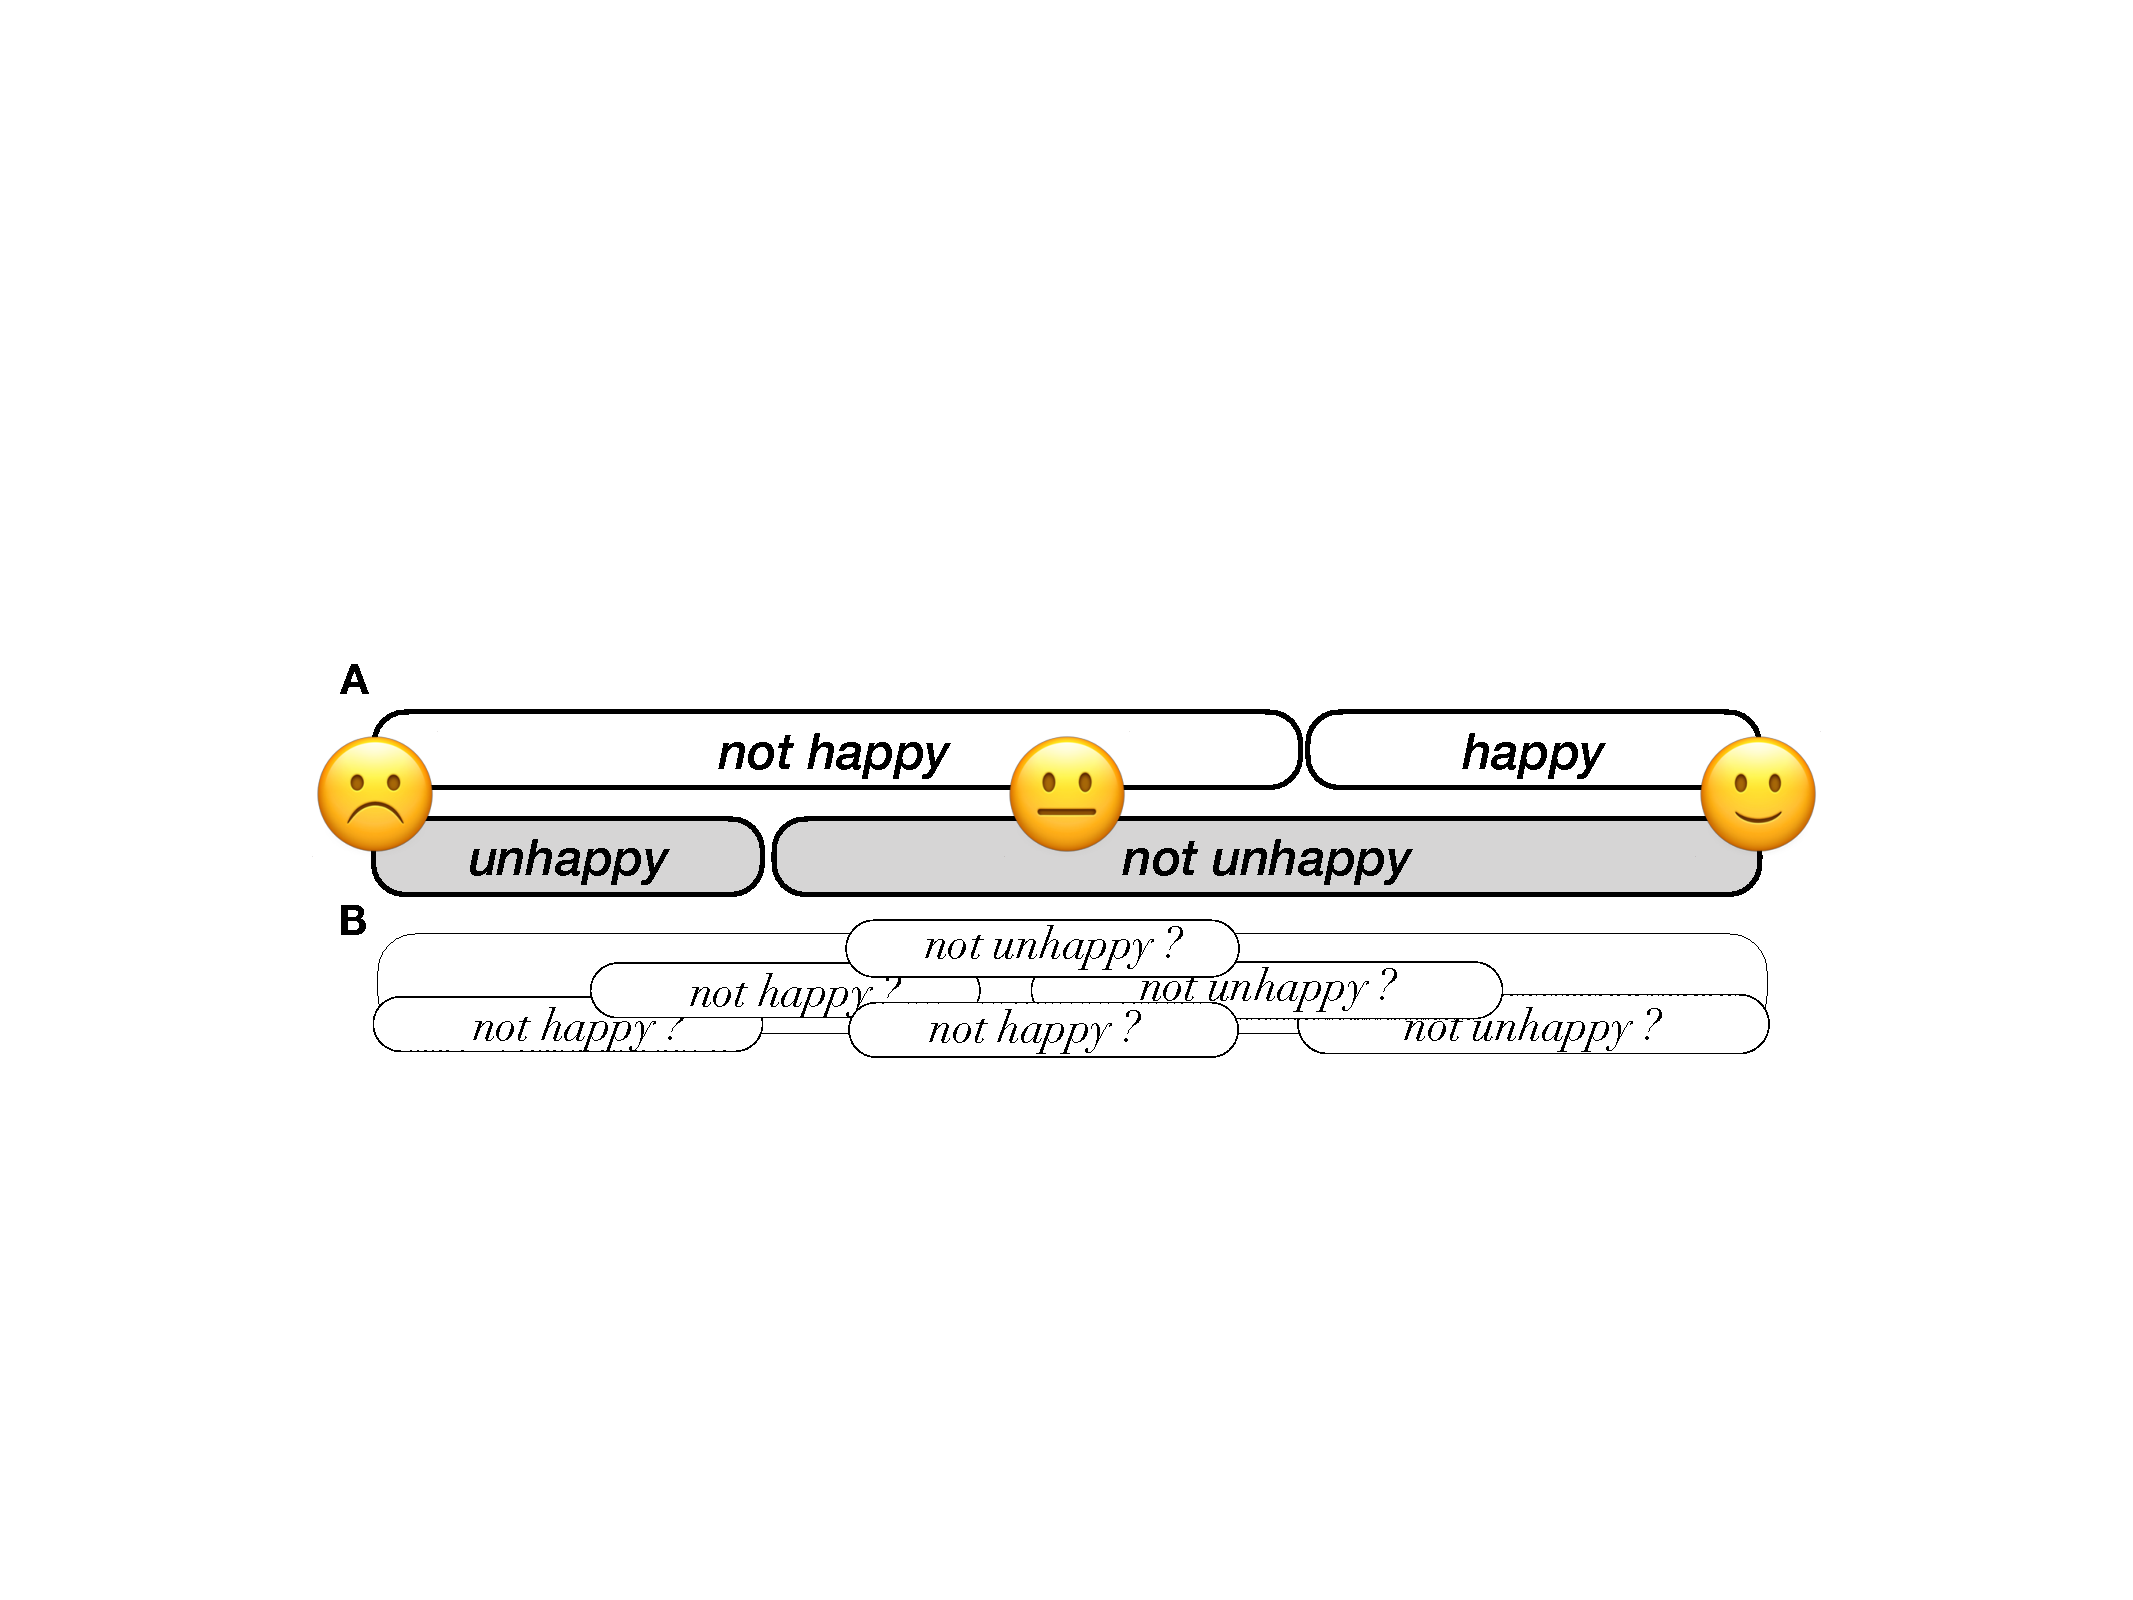
\includegraphics{figs/happy-scale-2}  
\caption{A: Theorized meanings of antonyms and their negations. B: How do listeners interpret \emph{not unhappy} and \emph{not happy}? }\label{fig:happy-scale}
\end{figure}

How does such a logical linguistic device---negation---give rise to a multiplicity of meanings?
Both syntactic \cite{Cable2017} and pragmatic \cite{Rett2014:eval} mechanisms have been proposed, but heretofore there have been no computational accounts tested against human behavioral data.
%In this paper, we 
%In addition, the ground truth as to the meaning of the language of negation has been left to the intuitions of trained theorists, who more often than not disagree on the basic facts. % come to different conclusions as to the meanings of these terms.
In this paper, we formalize and test the hypothesis that human listeners are uncertain about the meaning of negation, and that rational, communicative reasoning can be used to derive subtle meanings in the moment. 
Such an account points to a new avenue for exploitation by speakers: The meanings of logical words that explicitly convey negation carry a variety of interpretations.

\section{Modeling Double Negation}

Negation is the semantic operation of forming an opposite, but there is more than one way to convey an opposite. 
An integer must be either even or odd, because even and odd are \emph{contradictory} opposites: Contradictions cannot both be true but they also cannot both be false. 
On the other hand, a person could be tall, short, or neither tall nor short, because tall and short are \emph{contrary} opposites: Contraries cannot both be true but they can both be false. 
Formally, a contradictory opposition turns predicate $H$ into $\neg H$; contrary opposition turns $H$ into $\tilde{H}$. 
Contradictory opposition can be iterated ($\neg \neg H$) while contrary opposition cannot (i.e., $\tilde{\tilde{H}}$ is not a logical possibility;  \citeNP{Horn1989:Natural}).



% \(\neg \neg happy\) 
%The opposite of $(x > \theta_1)$ is either $(x \leq \theta_1)$ or $(x < \theta_2)$.



.\footnote{
Another example of iterated contradictory meaning is the intended meaning behind ``the enemy of my enemy is my friend''.
} 
%With these basic facts, we provide an informal description of our model before moving onto its formal characterization.
 %\red{(e.g., there is no unshort)}.\% \cite{Horn1989:Natural}.
%QAs a result, a single negative (\enquote{not happy} and \enquote{unhappy}) can mean either \(\neg happy\) or \(\tilde{happy}\), while double negatives (\enquote{not unhappy}) may mean \(\neg \neg happy\) or \(\neg \tilde{happy}\) (Fig.\(\thinspace\)\ref{fig:lexicon-model}).}

We propose that the logical distinction between contradictory~vs.~contrary opposition manifests in natural language markers (\enquote{not}, \enquote{un-}) in an unstable way.% and that  listeners maintain uncertainty about the mapping between logical negations and natural language negation% (\enquote{not}, \enquote{un-}) in a stable, context-invariant manner. 
%We imagine and resolve their uncertainty in context.  
A listener who hears statements involving negation reasons over a hypothesis space of logical possibilities (Figure \ref{fig:meanings}). 
Because contraries do not iterate, a double negative like \emph{not unhappy} could convey a double contradiction ($\neg \neg H$) or a contradiction about a contrary ($\neg \tilde{H}$): The former carries the same meaning as a positive adjective (\emph{happy}) whereas the latter conveys a distinct meaning. 
Intuitively, a rational speaker whose goal is to convey $H$ (or, $\neg \neg H$) would avoid the double negative construction because it is more verbose; thus, a sophisticated listener could backwards infer that a speaker who does use a double negative means to convey the expression with a unique meaning: $\neg \tilde{H}$.
This uncertain negation hypothesis further predicts that \emph{not happy} and \emph{unhappy} have the same set of possible meanings, and thus is not obvious whether the two expressions mean something distinct from one another. 
%\mht{he}
%This hypothesis further predicts that a listener who hears only a single adjective phrase in isolation (e.g., \enquote{unhappy}) has no basis from which to decide whether a contrary or contradiction was intended, and thus the listener should impart no meaning difference between an isolated .
%and thus a rational speaker would not have bothered to say \emph{not unhappy} (a more complex expression) if a double contradiction was their intention, so they likely were contradicting a contrary.

%This mutual-exclusivity kind of reasoning is also predicted to occur were a speaker to use two distinct negations in the same context (e.g., \enquote{Jones is not happy, while Smith is unhappy}, also Krifka's example above); that is, the model predicts that \emph{unhappy} is intended to convey more negative feelings than \emph{not happy} when the model observes the speaker using both kinds of negation in the same context.
%Thus, hearing a double negation does provide sufficient evidence to the listener that the speaker intends two different kinds of negation. 
%\mht{do we want to say here that we are looking at the negation of scalar adjectives, as opposed to other negation like phenomena?}
%Then, interpreting negated antonyms of scalar adjectives like \enquote{not unhappy} involves not only reasoning about negation but how various kinds of negation interact with the vagueness of scalar adjectives like \emph{happy} or \emph{tall}.


\begin{figure}[h]
\centering 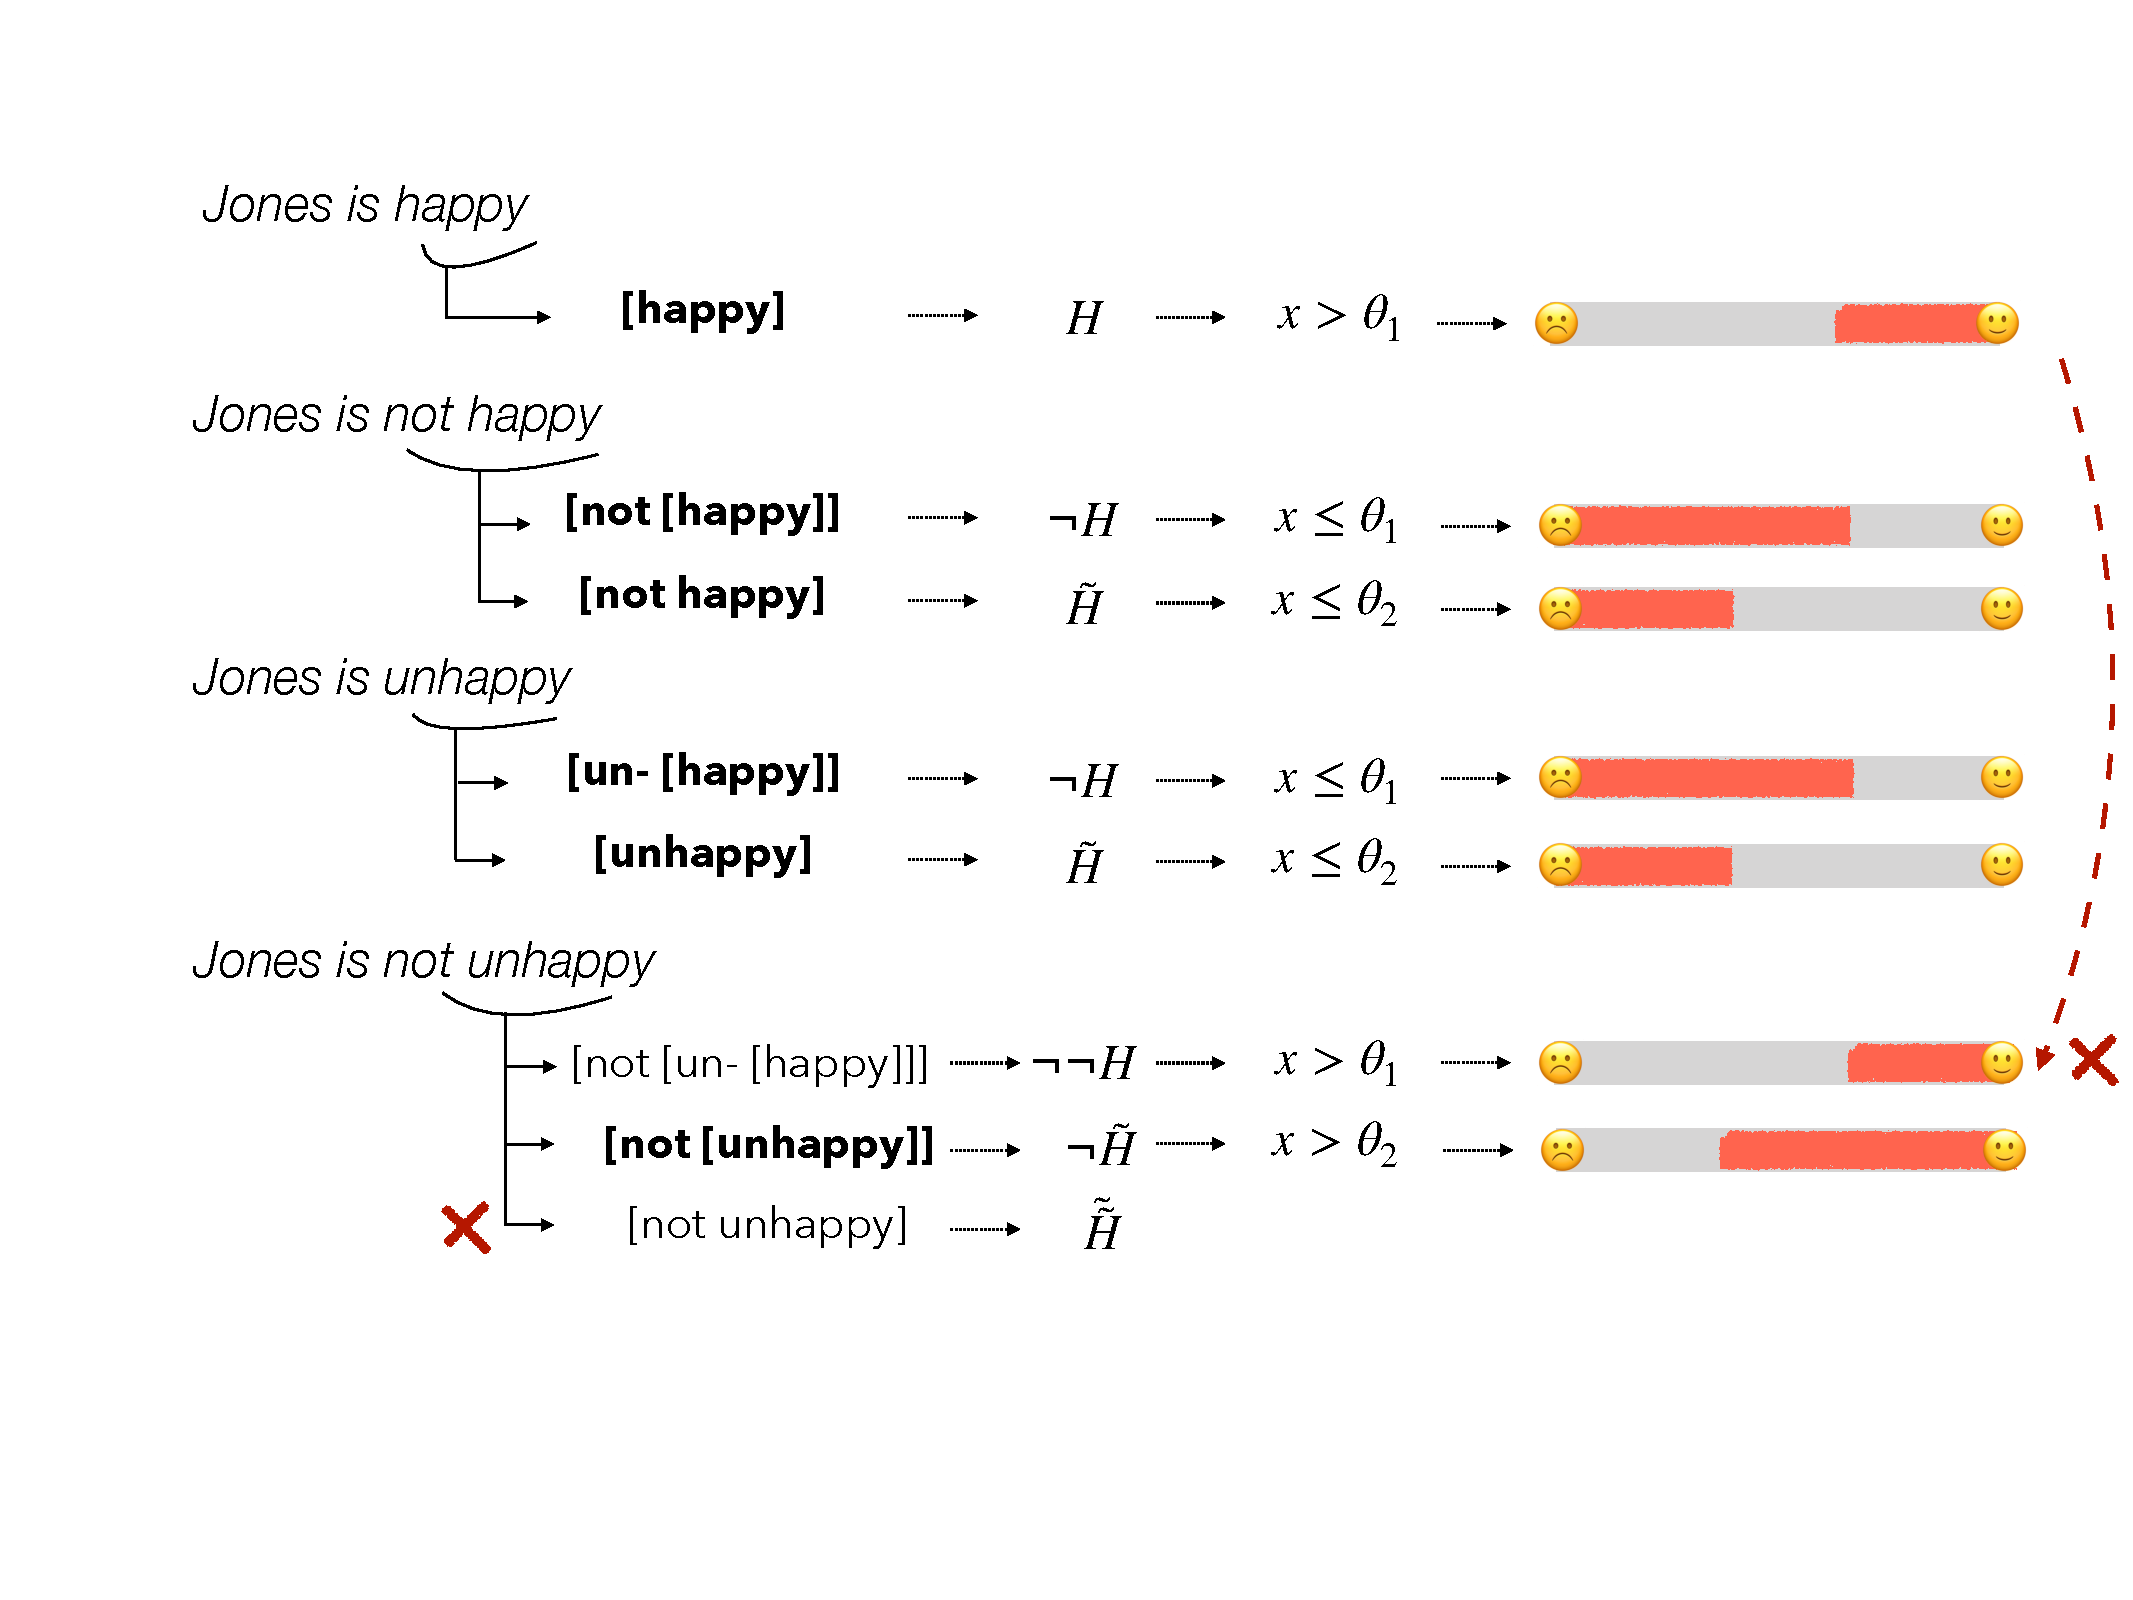
\includegraphics[width=0.8\textwidth]{figs/schematicMeanings}  
\caption{Set of possible meanings for antonym pairs and their negations for the uncertain negation model. 
Both ``not happy'' and ``unhappy'' could signal either contradictory $\neg H$ or contrary $\tilde{H}$ negation.
``Not unhappy'' can signal a double contradiction  $\neg \neg H$  or a contradiction of a contrary  $ \neg \tilde{H}$. A double contrary $\tilde{\tilde{H}}$ is not logically possible. A double contradiction  $\neg \neg H$  is pragmatically unlikely, because the same meaning is expressed by just the simple positive $H$. Scales on the right denote hypothetical interpretations of the different meanings.}
\label{fig:meanings}
\end{figure}

\mht{can we model this as an L2, where Lassiter adj model is modularized into $P(x \mid u, \mathcal{L})$ and we don't need to talk about thresholds?}
\begin{align}
P_L(x, \mathcal{L} \mid u) &\propto P_S(u \mid x, \mathcal{L}) \cdot P(x) \cdot P(\mathcal{L}) \\
P_S(u \mid x, \mathcal{L}) &\propto \exp{(\alpha \cdot \ln {P(x \mid u, \mathcal{L})} - \text{cost}(u))} \label{eq:S1}
\end{align}


%We hypothesize that \emph{lexical uncertainty}---uncertainty in the meaning of words---pervades even the language of logical devices, which interacts with conversational reasoning to give rise to a panoply of context-specific interpretations.
%Specifically, we posit that overt negation markers (\enquote{not}, \enquote{un-}) can convey different kinds of negation and that listeners resolve their uncertainty about the meaning in context.

We formalize this logic in a computational model drawing on the tools of formal semantics and probabilistic models of pragmatics \cite{Franke2015a, Goodman2016:RSA}. 
This formal model allows us to interrogate the conditions under which the above logic actually results in the interpretations we posit.
%; it also allows us to understand the contribution of the vagueness of predicates like \enquote{happy} or \enquote{tall} (i.e., that there is no single threshold beyond which a person qualifies as tall). 
Formally, a scalar adjective (e.g., \enquote{happy} or $H$) is thought to be literally true when the degree associated with that adjective \(x\) (e.g., the degree of happiness) is greater than some contextually-determined threshold \(\theta_1\): \(\mbox{ $[\![H]\!]$}(x, \theta_1): x > \theta_1\) \cite{Kennedy2007}.
%If a negation marker (e.g., \enquote{not}) creates a 
The contradictory opposite of such a meaning is simply that the degree is less than or equal to that same threshold: \(\neg \mbox{ $[\![H]\!]$}(x, \theta_1): x \leq \theta_1\).
The contrary opposite, on the other hand, creates a new predicate, which for a gradable adjective takes the form of a function with its own, distinct threshold \(\theta_2\): \(\mbox{ $[\![ \tilde{H} ]\!]$}(x, \theta_2): x \leq \theta_2\).
% which can in principle receive a different value than threshold $\theta_1$ for the positive adjective
If listeners are uncertain about how \enquote{not} and \enquote{un-} map onto these logical meanings, then negated positives like \enquote{not happy} and morphological antonyms like \enquote{unhappy} could in principle take either meaning. 
The hypothesis space of meanings for negated antonyms like \enquote{not unhappy} is constrained by the fact that contraries do not iterate; thus, negated antonyms either correspond to a double application of contradictory negation or a contradiction of a contrary. \footnote{``not un-H'' can then be either \(\neg \neg H\) or \(\neg (\tilde{H})\). Cashing these meanings out in terms of scalar adjectives, the order of operations need not matter: \(\neg (\tilde{H})\) $= \tilde{(\neg H)}$ , because both imply two sign-changes and one tokenization of a new threshold.}




%The act of producing a negated antonym (\enquote{not unhappy}) can then act as a signal towards the kinds of oppositions that the speaker had in mind (e.g., that the speaker intends to convey a contradictory negation of a contrary opposite).
%\mht{i think this point could be moved to a model implementation appendix or footnote}

%\red{Contradictory opposition can be iterated (\(\neg \neg Hx\)) but contrary opposition cannot \cite{Horn1989:Natural}.
%As a result, a single negative (\enquote{not happy} and \enquote{unhappy}) can mean either \(\neg happy\) or \(\tilde{happy}\), while double negatives (\enquote{not unhappy}) may mean \(\neg \neg happy\) or \(\neg \tilde{happy}\) (Fig.\(\thinspace\)\ref{fig:lexicon-model}).}

%In order to generate predictions, 
We embed these literal meanings in a probabilistic model of pragmatic reasoning, wherein a pragmatic listener $L_1$ resolves the meaning of an utterance $u$ by reasoning about why a rational speaker $S_1$ would have bothered to produce said utterance.
Eqs.~\ref{eq:L0}--\ref{eq:L1} describe a recursive Bayesian model in the Rational Speech Act tradition \cite{Franke2015a, Goodman2016:RSA}, in which the listener  has additional uncertainty about how their interlocutor (speaker $S_1$) uses negation markers to convey contradictory~vs.~contrary negations \cite{Bergen2016}.
We additionally take into account the vagueness of scalar adjectives using the technique proposed by \citeA{Lassiter2015} to derive thresholds \(\theta\) for interpreting vague adjectives (e.g., happy) in context:

%We formalize this as a prior distribution over possible lexica for the speaker $P(\mathcal{L})$.
%This model also takes into account the fact the scalar adjectives like \emph{happy} or \emph{tall} exhibit vagueness; i.e., there is no single, fixed $\theta$ beyond which the adjective is true. 
%---couched i---also a recursive reasoning model wherein a pragmatic listener \(L_{1}\) tries to resolve the intended meaning of an utterance \(u\) (e.g., \enquote{Jones is not unhappy}) by combining its prior beliefs about the degree of Jones' happiness \(P(x)\) with the Gricean assumption that speakers are generally cooperative \(S_1\) (Eqs.\(\thinspace\)\ref{eq:L1}-\ref{eq:L0}):
%Listener uncertainty about the interpretation of negation markers is modeled as uncertainty about the speaker's lexicon \(\mathcal{L}\) \cite{Bergen2016}.

\vspace*{-0.5cm}

\begin{align}
L_{0}(x \mid u, \theta, \mathcal{L}) &\propto \mathcal{L}(u, x, \theta) \cdot P(x) \label{eq:L0} \\
S_{1}(u \mid x, \theta, \mathcal{L}) &\propto \exp{(\alpha \cdot \ln {L_{0}(x \mid u, \theta, \mathcal{L})} - \text{cost}(u))} \label{eq:S1}\\
L_{1}(x, \theta, \mathcal{L} \mid u) &\propto S_{1}(u \mid x, \theta, \mathcal{L}) \cdot P(x) \cdot  P(\theta) \cdot P(\mathcal{L}) \label{eq:L1}
\end{align}

The literal listener \(L_0\) (Eq. \ref{eq:L0}) updates their prior beliefs over the degree \(P(x)\) via an utterance's literal meaning in lexicon \(\mathcal{L}\),
where \(\mathcal{L}(u, x, \theta)\) gives the truth-value of the utterance \(u\) in lexicon \(\mathcal{L}\) when applied to degree \(x\) (e.g., for $u= $\enquote{happy}, $\mathcal{L}$ returns a 1 when $x>\theta$ and a 0 when  $x\leq\theta$).
The speaker (Eq.~\ref{eq:S1}) is a soft-max rational agent (with degree of rationality  $\alpha$) who aims to act in accordance with a standard, information-theoretic utility function that tracks how well an utterance conveys the speaker's intended meaning $x$ to this literal listener---$\ln {L_{0}(x \mid u, \theta, \mathcal{L}}$)---while taking into account the cost of the utterance---$\text{cost}(u)$.
We assume that negation created by morphology (e.g., ``un-'' + happy) adds cost to the utterance as does creating a negation using the particle ``not'', and that the cost of ``un-'' is less than the cost of ``not''.\footnote{The uncertain negation model's qualitative predictions are sensitive to the exact values of the parameters. The predictions we show are invariant to cost so long as $\text{cost}(``un'') \leq \text{cost}(``not'')$ and $alpha$ is relatively small. Our goal is to show, under intuitively plausible parameter values, the uncertain negation model has the capacity to the make the predictions we describe; none of the alternative models we articulate have the capacity to make the unique predictions of the uncertain negation model.}
The intended meaning in this model is the value along a dimension referenced by an adjective (e.g., a degree of happiness).\footnote{
	This meaning is a special case of modeling meaning as a probability distribution over degrees of happiness (e.g., the speaker has only a rough sense of their personal degree of happiness), in which case the speaker's utility would be a function of the KL divergence between the literal listener's prior and posterior distributions over the degree given the utterance. 
}
The pragmatic listener (Eq.~\ref{eq:L1}) interprets an utterance by reasoning about three variables: the intended meaning or degree $x$, the threshold beyond which a scalar adjective is literally true  $\theta$, and the speaker's lexicon \(\mathcal{L}\) describing how the speaker uses negation. 
%, and the likelihood \(S_1(u \mid x, \theta, \mathcal{L})\) that a cooperative information-maximizing speaker would utter the adjective given a degree \(x\), threshold \(\theta\), and lexicon \(\mathcal{L}\).
%The speaker model \(S_1\) (Eq.\ref{eq:S1}) describes an approximately rational agent (with degree of rationality \(\alpha\)) trying to inform a naive listener \(L_0\) about the degree \(x\).


%\begin{figure}
%\centering
%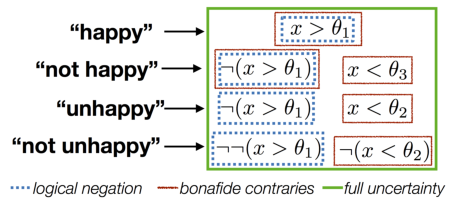
\includegraphics{figs/lexicon-model-1.pdf}
%\caption{\label{fig:lexicon-model}Space of possible meanings in the lexicon prior for the \emph{logical negation}, \emph{bonafide contraries}, and the full \emph{uncertain negation} models.}
%\end{figure}




We compare the predictions of this uncertain negation model to three theoretically-interesting, simpler alternative models.
First, we compare to a Vanilla RSA model which has neither lexical uncertainty about negation nor vagueness in the meaning of the adjective \cite{Frank2012}.\footnote{
The vanilla model assumes fixed-thresholds to the adjectives, and we assume antonyms convey contrary meanings. Therefore, we ascribe the following meanings to the adjectives: \enquote{happy} means \(>70\%\) on the happiness scale; \enquote{unhappy} means \(<30\%\).
}
Second, we compare to the Vague RSA model of \citeA{Lassiter2015}, assuming that all negation markers entail contradictory negation (the \emph{logical negation} or \emph{George Orwell} model).
Finally, we construct a \emph{bonafide contraries} model, building on \citeA{Lassiter2015}'s Vague RSA model by assuming morphological antonyms (\emph{un-}) convey contrary negation (e.g., \emph{unhappy} is to \emph{happy} how \emph{short} is to \emph{tall}) while the negation particular \emph{not} conveys contradictory negation.
%Finally, we construct fixed-threshold version of the Uncertain Negation model: this model is a lexical uncertainty model in the style of \citeA{Bergen2016}, which differs from our Uncertain Negation model only in its treatment of the semantics of the adjective as fixed as opposed to vague. 

\begin{table}[t]
\centering
\begingroup\fontsize{10pt}{11pt}\selectfont
\begin{tabularx}{\textwidth}{XXXXXXX}
\toprule
Model Name                    & Vagueness & Different negations & “happy”        & “un-”                            & “not ”                           \\ \midrule% & Description\\ \midrule
Vanilla RSA                   & No        & Yes                         & $x > 0.7$      & $x < 0.3$                        & $x < 0.7$                        \\% & Hard-coded contraries and contradictions \\
George Orwell                 & Yes       & No                          & $x > \theta$   & $x < \theta$                     & $x < \theta$                     \\% & Only Contradictions \\
Bonafide Contraries & Yes       & Yes                         & $x > \theta_1$ & $x  < \theta_2$                  & $x < \theta_1$                   \\% & Contraries and Contradictions \\
%Vanilla Lexical Uncertainty & No       & In Principle                         & $x > 0.7 $ & $x  < 0.3$ or   $x  < 0.7$              &  $x  < 0.3$ or   $x  < 0.7$                       \\% & Contraries and Contradictions \\
Uncertain Negation            & Yes       & In principle                & $x > \theta_1$ & $x  < \theta_2$ or $x < \theta_1$ & $x  < \theta_2$ or $x < \theta_1$ \\ %& Uncertain how “un” and “not” correspond with contrary vs. contradictory negation \\
\bottomrule
\end{tabularx}
\endgroup
\caption{Space of alternative models and the literal meanings they ascribe to negations.}
\end{table}



% Please add the following required packages to your document preamble:
% \usepackage{booktabs}

%{]}
%--\textgreater{}
A unique pattern of data is predicted by each model.
By design, the \emph{George Orwell} model does not distinguish different kinds of negation, and a double negation like \enquote{not unhappy} returns the same distribution as the positive adjective (\enquote{happy}).
When we hard-code different thresholds for \enquote{happy} and \enquote{unhappy} in the Vanilla RSA model, the model reasons that \enquote{not unhappy} does not communicate the same region of the space as \enquote{happy}; instead, the model restricts its interpretation to the neutral zone (i.e., \emph{not unhappy but not happy}); the same logic plays out for \enquote{not happy}, which receives the same neutral-feelings interpretation. 
The model that represents the vagueness of an adjective like \enquote{happy} and treats \enquote{unhappy} as a \emph{bonafide contrary} predicts the intuitive ordering expressed by \citeA{Krifka2007:Negated-antonyms}: \emph{unhappy} $<$ \emph{not happy} $<$ \emph{not unhappy} $<$ \emph{happy}, with \emph{not unhappy} receiving a slightly positive interpretation.
Finally, the full uncertain negation model predicts a different ordering: The uncertain negation model does not differentiate \enquote{unhappy} (antonyms) from \enquote{not happy} (negated positives), as \citeA{Jespersen1917:Negation} and \citeA{Blutner2004:pragmatics} surmised.
At the same time, upon hearing \enquote{not unhappy}, the \emph{uncertain negation} model reasons that a truly compositional \(\neg \neg \textit{happy}\) is implausible because the speaker could have just said the simpler \enquote{happy} and
interprets the utterance as signaling a slightly positive state (Fig.\(\thinspace\)\ref{fig:modelPredictions}).
%This pattern of judgments is uniquely predicted by the \emph{uncertain negation} model.
%The \emph{bonafide contraries} model also yields interpretations of negated antonyms as slightly positive, but predicts that \enquote{unhappy} (morphological antonym) signals a more negative state than \enquote{not happy} (negated positive).
%The \emph{logical negation} model does not differentiate between negated antonyms and positives, nor between negated positives and antonyms.




The \emph{uncertain negation} model's predictions are derived by reasoning about which lexicon best explains a speaker's utterance (Fig.\(\thinspace\)\ref{fig:modelPredictions}, \emph{single utterance}).
Hearing multiple utterances by the same speaker, however, can provide the listener more information about the speaker's lexicon, as in \citeA{Krifka2007:Negated-antonyms}'s example above (``I wasn't unhappy, just not happy''). 
The formal modeling approach we take here naturally allows for this extension by simply providing \(L_1\) with multiple adjective phrases; we condition each model on the observation of a speaker using all four adjective alternatives to describe different referents (e.g., \enquote{Sue is happy. Steve is not happy. Bill is unhappy. Barb is not unhappy.}; Fig.\(\thinspace\)\ref{fig:modelPredictions}, \emph{multiple utterances}).
Hearing multiple utterances has no effect on the Vanilla RSA model because it ascribes no uncertainty in meaning to the linguistic messages.
The models that do account for the vagueness of predicates derive more extreme differences in interpretations between utterances that could have different meanings (e.g., the difference between ``happy'' and ``not unhappy'' for \emph{Bonafide contraries} is greater when it hears multiple utterances).
This inference results from the fact that the listener has more evidence that the speaker intends different meanings for the different linguistic messages by virtue of the fact that the speaker used different messages.
Crucially, this inference results in the \emph{Uncertain negation} model predicting a meaning difference between \enquote{unhappy} and \enquote{not happy}: \enquote{unhappy} is more sad than \enquote{not happy}, producing the ordering hypothesized by \citeA{Krifka2007:Negated-antonyms} when both are used in the same context.
%All models have more extreme interpretations when they condition on multiple utterances.

\begin{figure}[t]
\centering 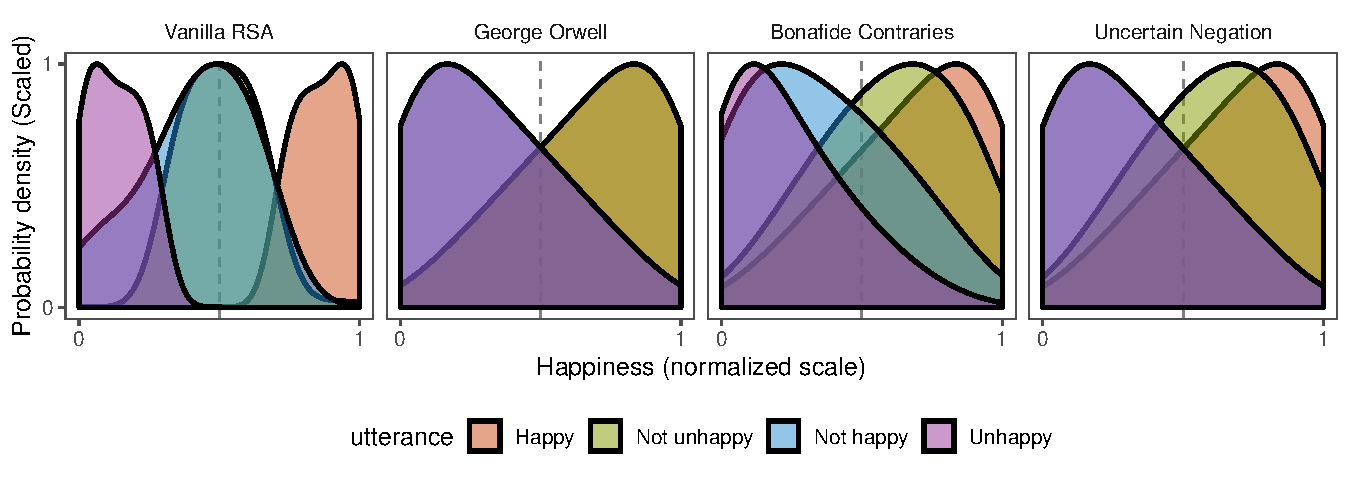
\includegraphics{figs/alternativeModels_dists.pdf} 
\caption{Model predictions for interpretations of antonym pairs and their negations. Model predictions use the following minimally assumptive model parameters: $P(x) = \text{Uniform}(0, 1); \alpha = 1; \text{cost}(\mathit{un}) = 2; \text{cost}(\mathit{not}) = 3$.}.\label{fig:modelPredictions}
\end{figure}

\section{Overview of Experiments}

The \emph{uncertain negation model} predicts a partial ordering for morphological antonyms and their negations when heard in isolation (with antonyms \(\approx\) negated positives), but a full ordering when present in the same context (Fig.\(\thinspace\)\ref{fig:modelPredictions}).
As a control condition, we examine antonyms which do not have overt negation markers (e.g., \emph{short}).
These lexical antonyms should behave like \emph{bonafide antonyms}, which predicts a full ordering regardless of context.
\text{Expt.$\thinspace$1} was exploratory and informed our computational modeling.
\text{Expt.$\thinspace$2} is a larger, more stringent, preregistered (\url{osf.io/p7f25/}) replication.
Finally, \text{Expt.$\thinspace$3} asks how specific the patterns of inferences are to morphological negation (\emph{un-}) as opposed to negation more broadly. 


\begin{table}[b]
\centering
\begingroup\fontsize{10pt}{11pt}\selectfont
\begin{tabularx}{\textwidth}{lll}
  \hline
 Adjective type & Definition & Examples \\ 
  \hline
 Positive & Positive-form scalar adjective & happy, mature \\ 
  Negated positive &  ``not'' + positive & not happy, not mature \\ 
  Morphological antonym &  Antonym created by morphology & unhappy, immature \\ 
  Lexical antonym & Antonym with a unique lexical item & sad, childish \\ 
  Negated morphological antonym &  ``not'' + morphological antonym & not unhappy, not immature \\ 
  Negated lexical antonym   &  ``not'' +  lexical antonym & not sad, not childish \\ 
  Negated negated positive  &  ``not'' + ``not'' + positive & not not happy, not not mature \\ 
   \hline
\end{tabularx}
\endgroup
\caption{Informal definitions and examples of adjective types investigated.} 
\end{table}

%\hypertarget{behavioral-experiments}




%\hypertarget{experiment-1-single-utterances}{%
%\subsection{Experiment 1: Single utterances}\label{experiment-1-single-utterances}
%}

\subsection{Methods}
%\hypertarget{participants}

We recruited 120 participants from Amazon's Mechanical Turk (MTurk).
This number was arrived at with the intention of getting approximately 25 ratings for each unique item in the experiment.
In all experiments, participants were restricted to those with U.S. IP addresses and at least a 95\% work approval rating; in addition, participants who self-reported a native language other than English were excluded.
The experiment took on average 3 minutes and participants were compensated \$0.40.

%\hypertarget{procedure}

On each trial, participants read a statement introducing a person using a gradable adjective of one of four \emph{adjective types}: positives (e.g., \emph{happy}, \emph{tall}), antonyms (e.g., \emph{short}, \emph{unhappy}), and their respective negations (\emph{not} X).
Antonyms were one of two types: morphological (e.g., \emph{unhappy}) and lexical (e.g., \emph{short}).
Participants rated the character on a scale from \enquote{the most \emph{positive} person} to \enquote{the most \emph{antonym} person} (item-dependent) using a slider bar (Fig.$\thinspace$\ref{fig:experiment-slides}A).
Participants rated one sentence at a time and saw items from both antonym types throughout the experiment.
Each participant completed a total of 16 trials, with exactly 2 repetitions of each adjective type for each antonym type.

%\hypertarget{materials}

We used adjectives that described properties of people.
We refer to a collection of the four associated adjective forms---positives, antonyms (morphological or lexical), and their negations using the particle \enquote{not}---that have the same positive adjective as an \emph{adjective set} (e.g., one adjective set is \emph{happy}, \emph{unhappy}, \emph{not happy}, \emph{not unhappy}).
10 adjective sets were constructed for each antonym type (total 20) from an informal survey of the linguistics literature and taken from a list of \enquote{common opposites} available online (Table 1).\footnote{\url{http://www.enchantedlearning.com/wordlist/opposites.shtml}}
Each trial of the experiment used an adjective from a distinct adjective set (e.g., if a participant rated \emph{unhappy}, they rated no other adjective from the \{\emph{happy}, \emph{unhappy}, \ldots{}\} set).

\begin{table}[h]
\centering
\begingroup\fontsize{10pt}{11pt}\selectfont
\begin{tabular}{ll}
  \hline
Morphological antonyms & Lexical antonyms \\ 
  \hline
attractive, unattractive & beautiful, ugly \\ 
  educated, uneducated & brave, cowardly \\ 
  friendly, unfriendly & fat, skinny \\ 
  happy, unhappy & hard-working, lazy \\ 
  honest, dishonest & loud, quiet \\ 
  intelligent, unintelligent & proud, humble \\ 
  interesting, uninteresting & rich, poor \\ 
  mature, immature & strong, weak \\ 
  polite, impolite & tall, short \\ 
  successful, unsuccessful & wise, foolish \\ 
   \hline
\end{tabular}
\endgroup
\caption{Items in Experiment 1.} 
\end{table}

%\hypertarget{results}

6 participants were excluded for self-reporting a native language other than English, leaving a remainder of 114 participants for these analyses, which resulted in on average 23 ratings for each unique adjective in our stimulus set.
The qualitative predictions of our models concern the ordering within a set of alternatives for different antonym types (morphological vs.~lexical).
%To visualize the data, we compute normalized responses on a participant-wise basis (i.e., normalized response \(r'_{ij} = \frac{r_{ij} - mean_j}{sd_j}\) for trial \(i\) and participant \(j\)).
Fig.$\thinspace$\ref{fig:expt1-results} shows the empirical distributions for each of the four adjective types for both morphological and lexical antonyms adjective sets.
Critically, as predicted by the uncertain negation model, adjective sets with morphological antonyms show only a partial ordering, while those with lexical antonyms show a full ordering.

To confirm these observations, we built a linear mixed model predicting the raw, unnormalized ratings in terms of fixed effects of \emph{antonym type} (morphological vs.~lexical), \emph{adjective type} (Helmert coded in order: antonym, negated positive, negated antonym, positive)\footnote{Throughout, we code adjective type using Helmert coding, which compares levels of a factor to the average of preceding levels, in order to compare antonym vs.~negated positive levels of the adjective type factor.}, and their interaction; the model also included random intercepts and random slopes of \emph{adjective type} by-participant and by-item.\footnote{This, and all subsequent regression models, were the maximal mixed-effects model that converged for the data set that additionally explained significantly more variance than models with simpler mixed-effects structures, using the \texttt{lme4} package in R \cite{lme4}.}
Consistent with our observations, the difference between the \emph{antonym} vs. \emph{negated positive} levels of adjective type interacted significantly with antonym type (morphological vs.\text{~}lexical; \(\beta = 0.03\), t\((16) = 2.40, p = 0.03\)).

We also observe that negated morphological antonyms (e.g., \emph{not unhappy}) were rated lower than negated lexical antonyms (e.g., \emph{not tall}; Fig.$\thinspace$\ref{fig:expt-results}A).
Closer investigation of responses revealed that negated antonyms (and not other adjective types) received a bimodal distribution: Most ratings were slightly positive but a clearly distinguishable minority distribution of ratings were slightly negative (e.g., \emph{not dishonest} meaning \emph{not honest}).
This weakly negative interpretation for negated antonyms was present at least somewhat in every item and in most participants.
This interpretation may be the result of participants attributing politeness to the speaker: \emph{Not dishonest} may be an indirect way of saying that a person is not honest (Yoon, Tessler, Goodman, \& Frank, 2017).

\begin{figure}[hbt]

{\centering 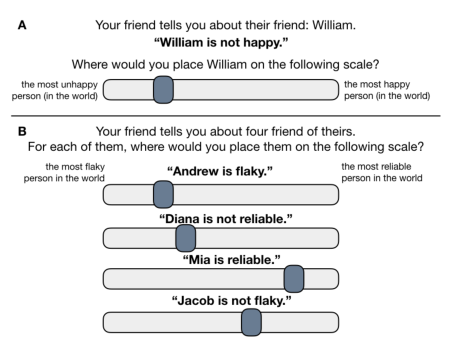
\includegraphics[width=0.7\linewidth]{figs/experiment-slides-1} 

}

\caption{Example experimental trials for (A) single utterance (Expts. 1, 2) and (B) multiple utterances (Expts. 2, 3) conditions. ``in the world'' wording for endpoints was used in Expts. 2 \& 3. (A) shows a trial from a morphological antonym set while (B) shows a lexical antonym set.}\label{fig:experiment-slides}
\end{figure}

\begin{figure*}[h]
\centering 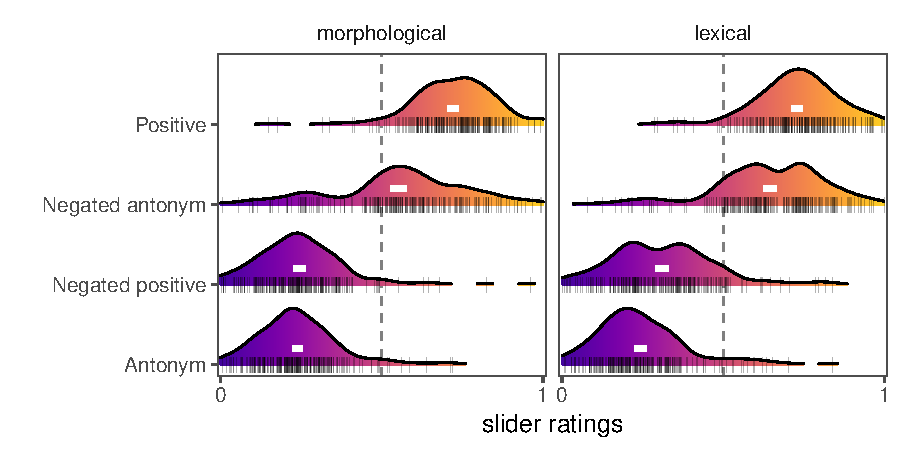
\includegraphics[width=0.95\linewidth]{figs/expt1_ridges_wCIs} 
\caption{Experiment 1 results. Empirical distributions of responses for adjective sets with morphological antonyms (e.g., ``unhappy'') and lexical antonyms (e.g., ``sad''). Dashed line indicates the midpoint of the scale. Dashes below density plots denote individual responses. White bars denote bootstrapped 95\% confidence intervals.}\label{fig:expt1-results}
\end{figure*}

%\hypertarget{experiment-2-single-and-multiple-utterances}

\text{Expt.$\thinspace$1} revealed an asymmetry: Lexical antonyms (e.g., \emph{short}) were clearly distinguished from negated positives (e.g., \emph{not tall}), whereas morphological antonyms were not (e.g., \emph{unhappy} \(\approx\) \emph{not happy}).
In \text{Expt.$\thinspace$1}, our adjective sets varied both in terms of their antonym type (morphological vs.\text{~}lexical) as well as the actual degree scales being described (e.g., height for \emph{tall}/\emph{short} vs.\text{~}happiness for \emph{happy}/\emph{unhappy}).
Many adjective sets have both morphological and lexical antonyms (e.g., \emph{happy}/\emph{unhappy}/\emph{sad}).
Here, we aim to replicate the asymmetry findings using adjectives that describe the same semantic scales.
Also, we test our second prediction that hearing multiple utterances in the same context will produce the full ordering for morphological antonym sets (Fig.\(\thinspace\)\ref{fig:modelPredictions}).

\subsection{Methods}
%\hypertarget{participants-1}

We recruited 750 participants from MTurk.
The experiment comprised of four between-subjects experimental conditions arranged in a 2x2 design: \emph{antonym type (morphological vs.\text{~}lexical)} X \emph{context (single vs.\text{~}multiple utterances)}.
300 participants were assigned to each \emph{antonym type} in the \emph{single utterance} contexts, and 75 participants were assigned to each in the \emph{multiple utterances} conditions.
These numbers follow from the intention of getting approximately 45 ratings for each unique adjective in the experiment.
The \emph{single utterance} task took on average 3 minutes and participants were compensated \$0.40; \emph{multiple utterances} took on average 5 minutes and participants were compensated \$0.80.
Exclusion criterion, sample size, procedure, and the analysis described below were preregistered: \url{osf.io/p7f25/}.

%\hypertarget{materials-1}

To best isolate the contribution of morphological vs.\text{~}lexical antonyms, we curated adjective sets consisting of words for properties of people, such that both types of antonyms existed for the same positive adjective (e.g., \emph{happy} \(\rightarrow\) \emph{unhappy}, \emph{sad}; \text{Table$\thinspace$2}).
Lexical antonyms were selected from a set of possibilities produced from a small survey (n=18) on MTurk eliciting \enquote{opposites} for a list of 30 positive-form adjectives which had morphological antonyms (asking participants in the same experimental context as our interpretation studies, \enquote{What is the opposite of e.g., \emph{forgiving}?}).
From the list of freely-produced opposites (the vast majority of which were not morphological), the first author chose the one that intuitively best conveyed the same scalar dimension as the morphological antonym and which was not already used as a lexical antonym for another item (e.g., opposite of \emph{forgiving} \(\rightarrow\) \emph{resentful}; opposite of \emph{kind} \(\rightarrow\) \emph{cruel}, because opposite of \emph{friendly} \(\rightarrow\) \emph{mean}).
Ten out of the original 30 items were dropped for either not having such a well-suited lexical antonym (e.g., \emph{moral}) or for having a well-suited lexical antonym that conflicted with another item (e.g., \emph{compassionate} \(\rightarrow\) \emph{cold}, but also \emph{affectionate} \(\rightarrow\) \emph{cold}).

%\hypertarget{procedure-1}

In the \emph{multiple utterances} conditions, participants rated all four adjective types simultaneously, each referring to a different person (Fig.$\thinspace$\ref{fig:experiment-slides}B), for a total of 12 trials.
The \emph{single utterances} conditions were similar to that of \text{Expt.$\thinspace$1}: Participants rated one sentence at a time (e.g., \enquote{Greg is not unhappy}), each from a unique adjective set (e.g., never rated both \emph{unhappy} and \emph{not happy}), completing a total of 12 trials, with exactly 3 repetitions of each adjective type (positive, antonym, and their negations).
In contrast to \text{Expt.$\thinspace$1}, \emph{antonym type} (morphological vs.\text{~}lexical) was a between-participants factor.
In addition, the slider bar endpoints were relabeled to \enquote{the most \{\emph{positive}, \emph{negative}\} person \emph{in the world}}; without \enquote{in the world}, there is a salient interpretation of the endpoints indicating \enquote{the most \{\emph{positive}, \emph{negative}\} person (of these four)} in the multiple utterances conditions.

\begin{table}[h]
\centering
\begingroup\fontsize{9pt}{10pt}\selectfont
\begin{tabular}{lll}
  \hline
Positive adjective & Morphological antonym & Lexical antonym \\ 
  \hline
affectionate & unaffectionate & cold \\ 
  ambitious & unambitious & lazy \\ 
  attractive & unattractive & ugly \\ 
  educated & uneducated & ignorant \\ 
  forgiving & unforgiving & resentful \\ 
  friendly & unfriendly & mean \\ 
  generous & ungenerous & stingy \\ 
  happy & unhappy & sad \\ 
  honest & dishonest & deceitful \\ 
  intelligent & unintelligent & stupid \\ 
  interesting & uninteresting & boring \\ 
  kind & unkind & cruel \\ 
  mature & immature & childish \\ 
  patriotic & unpatriotic & traitorous \\ 
  polite & impolite & rude \\ 
  rational & irrational & crazy \\ 
  reliable & unreliable & flaky \\ 
  resourceful & unresourceful & wasteful \\ 
  sincere & insincere & fake \\ 
  tolerant & intolerant & bigoted \\ 
   \hline
\end{tabular}
\endgroup
\caption{Items used in Experiment 2.} 
\end{table}

%\hypertarget{results-1}

35 participants were excluded for self-reporting a native language other than English, leaving 715 participants for these analyses.
Results for each adjective type in each condition are shown in Fig.$\thinspace$\ref{fig:expt2-results}.


\begin{figure*}[h]
\centering 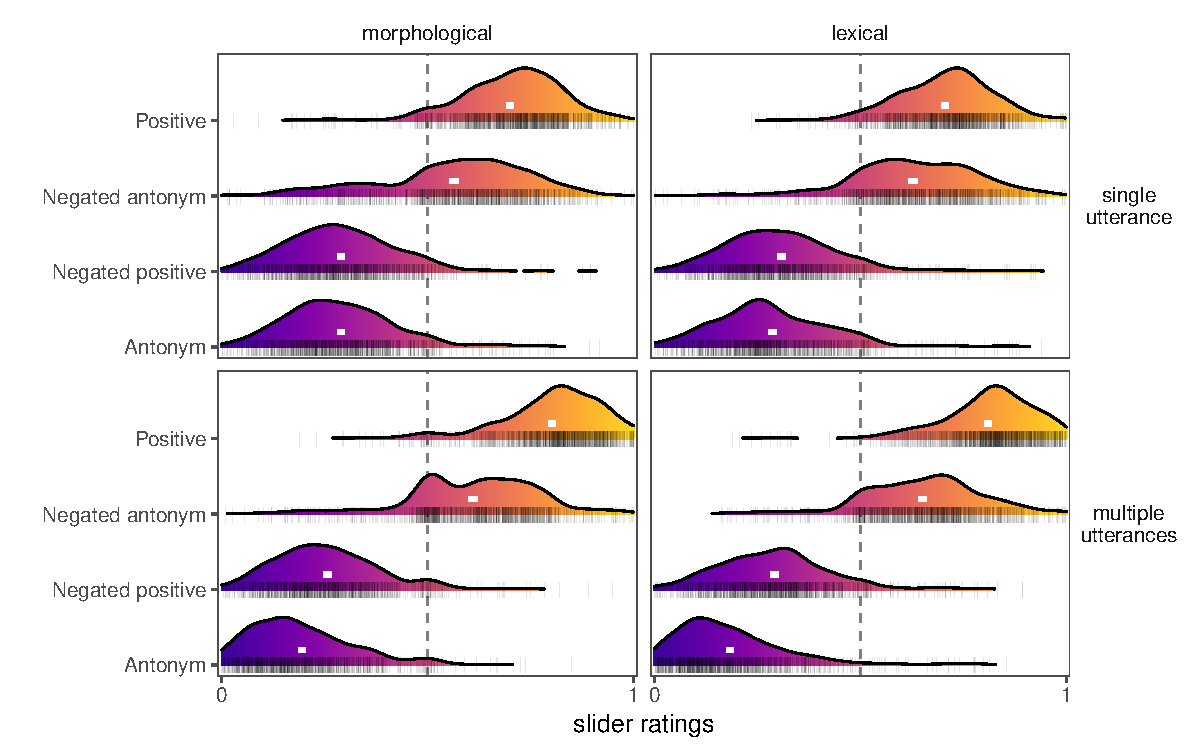
\includegraphics[width=0.95\linewidth]{figs/expt2_ridges_wCIs} 
\caption{Experiment 2 results. Empirical distributions of responses for adjective sets with morphological antonyms (e.g., ``unhappy'') and lexical antonyms (e.g., ``sad'') for the single utterance and multiple utterances conditions. Dashed line indicates the midpoint of the scale. Dashes below density plots denote individual responses. Width of white rectangles denotes bootstrapped 95\% confidence intervals.}
\label{fig:expt2-results}
\end{figure*}

As we did in \text{Expt.$\thinspace$1}, we evaluate our hypothesis that morphological antonyms behave like the \emph{uncertain negation} model (i.e., show a partial ordering) while lexical antonyms show a true ordering (like \emph{bonafide contraries}).
We considered data only from the \emph{single utterances} conditions and built a linear mixed model predicting the unnormalized ratings in terms of \emph{antonym type} (morphological vs.\text{~}lexical), \emph{adjective type} (Helmert coded in order: antonym, negated positive, negated antonym, positive) and their interaction; the model also included random intercepts and random slopes of \emph{adjective type} by-participant and by-item.
Consistent with our hypothesis, the interaction between the \emph{antonym} vs.\text{~}\emph{negated positive} levels of adjective type and antonym type (morphological vs.\text{~}lexical) was significant (\(\beta = 0.01\), t\((565) = 2.68, p = 0.01\)).
We then analyzed the simple effects.
Morphological antonyms were not significantly different than negated positives (\(\beta = 5.3e-05\), t\((52) = 0.02, p = 0.98\)), while lexical antonyms were interpreted more negatively than negated positives (\(\beta = -0.01\), t\((280) = 3.66\),
\(p = 0.00\)).\footnote{The random effect structure for the simple effects models mirrored the full model. The only difference was that in analyzing the lexical antonyms, the random effect of adjective type by-item needed to be dropped in order for the model to converge.}

Our second main hypothesis is that context (single vs.\text{~}multiple utterances) modulates the interpretive difference between morphological antonyms and negated positives.
Specifically, we predict that morphological antonyms will be interpreted more negatively than negated positives in a context with multiple utterances.
To evaluate this hypothesis, we considered data only from the morphological antonyms conditions and built a linear mixed model predicting the raw, unnormalized ratings in terms of adjective type,
context (single vs.~multiple utterances) and their interaction; the model also included random intercepts and random slopes of adjective type by-participant and by-item.
This interaction was also significant (\(\beta = 0.03\), t\((6457) = 6.73, p = 1.9e-11\)), and in the correct direction (see Fig.\text{~}\ref{fig:expt2-results}).

The predictions of the \emph{uncertain negation} model are ambiguous about the relevant three-way interaction ( \emph{antonym} vs. \emph{negated positive} by lexical vs. morphological adjective type by context).
On the one hand, for the \emph{antonym} vs. \emph{negated positive} contrast, the model predicts no difference in meaning for morphological antonyms when presented in isolation, but does does predict meaning differences when the alternatives are presented together, whereas the difference is expected to occur for lexical antonyms in both context conditions.
On the other hand, the model's inferences about the likely meaning of all of the adjectives gets further differentiated as a result of being presented in the same context (i.e., all adjectives get more specific interpretations).
Thus, it is not clear \emph{a priori} that the model predicts a three-way interaction nor the direction of the interaction.
Thus, as an exploratory analysis, we examined these effects in a full three-way interactive model, and the found the relevant three-way interaction was in the direction of lexical antonyms showing a larger \emph{antonym} vs. \emph{negated positive} difference in the explicit context; this effect was not significant (\(\beta = 0.01\), t\((469) = 1.64, p = 0.1\)).

\section{Experiment 3: Blatant double negatives}\label{experiment-3-notnot}

In this last experiment, we test whether the slightly positive interpretation of negated antonyms (``not unhappy'') is the result of a specific characteristic of morphological negation (\emph{un-}) or a property of the uncertain status of negation markers more generally. 
We do this by testing interpretations of blatantly double negative statements that use modifier negation twice (``not not happy'').
%In addition, we test the limits of contextual differentiation of meaning by simultaneously presenting participants with negated antonyms (``not unhappy''). 
We use the \emph{multiple utterances} context in order to maximize the possibility of detecting meaning differences. 

\subsection{Methods}

\subsubsection{Participants}\label{participants-3}

We recruited 75 participants from MTurk to match the sample size of the same condition in Expt.~2.
These numbers follow from the intention of getting approximately 45 ratings for each unique adjective in the experiment.
The experiment took on average 5 minutes and participants were compensated \red{\$0.80.}
\red{Exclusion criterion, sample size, procedure, and the analysis described below were preregistered: \url{osf.io/p7f25/}.}

\subsubsection{Materials and procedure}\label{materials-3}

The materials and procedure were identical to that of the \emph{multiple utterances} condition of Expt.~2.
The only difference in this experiment is that participants are presented with the following alternatives: positives, negated positives, morphological antonyms, and negated negated positives (e.g., \emph{happy}, \emph{not happy}, \emph{unhappy}, \emph{not not happy}).

\subsection{Results}

\red{X} participants were excluded for self-reporting a native language other than English, leaving \red{Y} participants for these analyses.
Results for each adjective type are shown in Figure \ref{fig:expt3-results}.

Our main hypothesis concerns the interpretation of blatantly double negative statements that use the same negation marker twice (``not not happy''). We predict that on average, interpretations will be substantially above the midpoint of the scale (i.e., double negatives receive a slightly positive interpretation) and substantially below the ratings for the positive adjective (``happy''). 


\begin{figure*}[h]
\centering 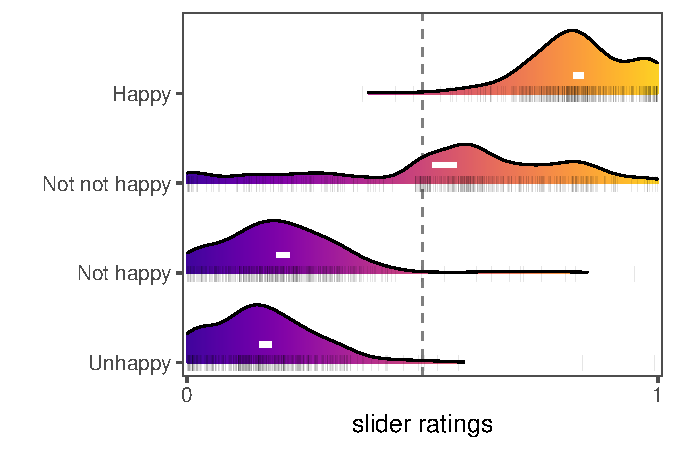
\includegraphics[width=0.95\linewidth]{figs/expt3_ridges_wCIs} 
\caption{\red{[Pilot data]} Experiment 3 results. Empirical distributions of responses for adjective sets with morphological antonyms (e.g., ``unhappy'') and lexical antonyms (e.g., ``sad''). Dashed line indicates the midpoint of the scale. Dashes below density plots denote individual responses. White bars denote bootstrapped 95\% confidence intervals.}\label{fig:expt3-results}
\end{figure*}


%\hypertarget{discussion}{%
\section{Discussion}\label{discussion}

%\mht{Discuss Horn's analysis as division of pragmatic labor. Does the fact that we need some cost for this to get off the ground provide some resonance for Horn (1991)'s analysis?}
%}
%\mht{this opening paragraph is more about vagueness than uncertain negation...}
%Many dimensions that language can pick out have no units.
%Speakers cannot say they are \emph{42 units happy} like they can say they are \emph{6'1" tall}.
%Instead, speakers can use modifiers and morphemes to carve more precise meanings from otherwise vague dimensions.
%A person \emph{not unhappy} is neither sad nor truly happy, but residing in some marginally positive state that is difficult to refer to because degrees of happiness lack precise units.

This paper provides a computational solution to an outstanding puzzle in natural language understanding: How to interpret double negatives (e.g., \emph{not unhappy}; Krifka, 2007; Rett, 2014).
We additionally discovered and confirmed a surprising empirical result that challenges ``established'' intuitions in linguistics: \emph{unhappy} and \emph{not happy} are not immediately differentiated, except when both are present in the same context.
Our model that represents uncertainty about how to interpret overt negation markers (\emph{un-}, \emph{not}) predicts this very result, while alternative models that treat negation markers as only carrying a single possible meaning fall short.

It is noteworthy that we are able to recover, both in our model and empirically, the ordering predicted by Krifka (2007) for morphological antonyms when a listener hears multiple adjectival utterances in the same context (\emph{multiple utterances condition}).
This work thus carries with it an account of a robust linguistic intuition: Potentially equivalent expressions receive differential interpretations when observed uttered by the same speaker in close proximity.
Reasoning about lexical ambiguity, listeners conclude that a choice of different expressions may be most likely for a speaker who differentiates meanings.
More generally, the inferences modeled here can be seen as an instance of \emph{mutual exclusivity} (Markman, 1989), in which listeners resolve uncertainty about multiple elements of meaning simultaneously.

In our final experiment, we showed that blatantly double negative statements such as \emph{not not happy} receive an interpretation similar to that of more conventional negated antonyms (\emph{not unhappy}) as indicating a slightly positive state. 
The fact that \emph{not not happy} is differentiated in meaning from the simple \emph{happy} suggests the same word (\emph{not}) can be interpreted in two different ways (i.e., conveying contradictory~vs.~contrary negation) within a single utterance. 
This result suggests a radical view of uncertainty about negation markers, where the uncertainty is not only resolved at the level of individual speakers but that it can be computed for each individual usage of a word.
%At the same time, expressions of double negation (\emph{not not}, \emph{not un-}) were not differentiated by listeners even when presented in the same context, suggesting that language understanding respects the logical possibilities that the rules of semantic opposition permit  \cite{Horn1989:Natural}.
%These results suggest both a radical but bounded view of the uncertainty of linguistic expressions. 

Our formalization of lexical uncertainty about the meaning of natural language negation builds on a growing movement to treat the combinatorial rules of grammar as not totally separable from the lexicon (e.g., Bybee, 2006; O'Donnell, 2015).
Recent psycholinguistic evidence supports the idea that utterances which are heavily used will be processed as unique lexical entries while less frequent phrases will be understood compositionally (Morgan \& Levy, 2016).
The two types of negation meaning we considered---contrary and contradictory opposition---can be seen as a \emph{lexicalized} form of opposition (with the adjective receiving its own threshold variable) and a \emph{compositional} rule (logical negation), respectively.
In our modeling, we assumed all lexica (all logically-possible interpretations of negation) were equally likely \emph{a priori}: A further test of our negation uncertainty model would be to see if frequency can serve as a proxy for this prior over lexica.

In this paper, we aimed to explain the modal interpretations of antonym pairs and their negations, but both intuition and our empirical data suggest more nuance and variability in judgments.
Consistently across our experiments, we found that negated antonyms received a modal interpretation that is slightly positive; at the same time, negated antonyms reliably elicited a slightly negative interpretation as well (e.g., the meaning expressed by ``he's not [un]reliable \emph{but he is kind of flaky}'', with prosodic focus on [un-]).
This interpretation may be the result of participants attributing politeness to the speaker: Not unreliable may be an indirect way of saying that a person is not reliable \cite{Yoon2017}.
There are also examples dating back to at least \red{Bolinger (1972)} that point the usage of double negatives in understatement: In the appropriate context, ``I was not unaware of the problem'' could mean \emph{I was damn well aware of the problem}; we do not find any evidence that such interpretations were garnered in our experiments. 
%\red{[Horn ``not unaware'']}
%\red{[midpoint responses? ]}
All our experiments involve utterances conveyed in text with minimal contexts; future work should investigate the relevant context and prosodic cues that can be used to derive diverse interpretations from antonym pairs and their negations.

To negate is to make true false, but for statements that are truly vague, the behavior of negation is not so obvious.
We present a computational explanation for why this is so, and provide empirical data that sheds new light on the age old question of meaning and opposition.

%\mht{other thoughts: (a) dimensionality in antonyms (unhappy and sad map onto slightly different dimensions); (b) how much of this is specific to (American) English? [there is an oft intuition that Orwell believes this because he is british]; (c) relation to understatement more broadly}


%This result suggests a radical uncertainty model, where the meanings of linguistic expressions are computed on the fly
%Our final experiment challenges rigid views of language 
%One limitation of this work is that we stipulate, rather than derive, differences in meaning for morphological vs.~lexical antonym pairs (cf., Rett, 2014).


\newpage

%\hypertarget{references}{%
%\section{References}\label{references}%}



\bibliographystyle{apacite}

\setlength{\bibleftmargin}{.125in}
\setlength{\bibindent}{-\bibleftmargin}

\bibliography{negant}
%
%\begingroup
%\setlength{\parindent}{-0.5in}
%\setlength{\leftskip}{0.5in}
%
%\hypertarget{refs}{}
%\leavevmode\hypertarget{ref-lme4}{}%
%Bates, D., M\wrapmf{\"{a}}chler, M., Bolker, B., \& Walker, S. (2015). Fitting linear mixed-effects models using lme4. \emph{Journal of Statistical Software}, \emph{67}(1), 1--48.
%
%\leavevmode\hypertarget{ref-Bergen2016}{}%
%Bergen, L., Levy, R., \& Goodman, N. D. (2016). Pragmatic reasoning through semantic inference. \emph{Semantics and Pragmatics}, \emph{9}.
%
%\leavevmode\hypertarget{ref-Blutner2004:pragmatics}{}%
%Blutner, R. (2004). Pragmatics and the lexicon. \emph{Handbook of Pragmatics}, \emph{488514}.
%
%\leavevmode\hypertarget{ref-bybee2006usage}{}%
%Bybee, J. L. (2006). From usage to grammar: The mind's response to repetition. \emph{Language}, \emph{82}(4), 711--733.
%
%\leavevmode\hypertarget{ref-Cable2017}{}%
%Cable, S. (2017). The good, the 'not good', and the 'not pretty': Negation in the negative predicates of tlingit.
%
%\leavevmode\hypertarget{ref-Franke2015a}{}%
%Franke, M., \& J\wrapmf{\"{a}}ger, G. (2015). Probabilistic pragmatics, or why Bayes' rule is probably important for pragmatics. In \emph{Zeitschrift für sprachwissenschaft} (pp. 3--44).
%
%\leavevmode\hypertarget{ref-Goodman2016:RSA}{}%
%Goodman, N. D., \& Frank, M. C. (2016). Pragmatic language interpretation as probabilistic inference. \emph{Trends in Cognitive Sciences}, \emph{20}(11), 818--829.
%
%\leavevmode\hypertarget{ref-Horn1989:Natural}{}%
%Horn, L. R. (1989). \emph{A natural history of negation}. University of Chicago Press.
%
%\leavevmode\hypertarget{ref-Horn1991:Duplex}{}%
%Horn, L. R. (1991). Duplex negatio affirmat...: the economy of double negation. \emph{CLS 27-II: Papers from the Parasession on Negation}, 80--106.
%
%\leavevmode\hypertarget{ref-Jespersen1917:Negation}{}%
%Jespersen, O. (1917). \emph{Negation in english and other languages}. Kobenhavn: Host.
%
%\leavevmode\hypertarget{ref-Jespersen1924}{}%
%Jespersen, O. (1924). \emph{The philosophy of grammar}. London: Allen \& Unwin.
%
%\leavevmode\hypertarget{ref-Kennedy2007}{}%
%Kennedy, C. (2007). Vagueness and grammar: the semantics of relative and absolute gradable adjectives. \emph{Linguistics and Philosophy}, \emph{30}, 1--35.
%
%\leavevmode\hypertarget{ref-Krifka2007:Negated-antonyms}{}%
%Krifka, M. (2007). Negated Antonyms: Creating and Filling the Gap. \emph{Presupposition and Implicature in Compositional Semantics}, 163--177.
%
%\leavevmode\hypertarget{ref-Lassiter2015}{}%
%Lassiter, D., \& Goodman, N. D. (2015). Adjectival vagueness in a Bayesian model of interpretation. \emph{Synthese}.
%
%\leavevmode\hypertarget{ref-Markman1989}{}%
%Markman, E. M. (1989). \emph{Categorization and naming in children: Problems of induction}. MIT Press.
%
%\leavevmode\hypertarget{ref-MorganLevy2016:binomials}{}%
%Morgan, E., \& Levy, R. (2016). Abstract knowledge versus direct experience in processing of binomial expressions. \emph{Cognition}, \emph{157}, 384--402.
%
%\leavevmode\hypertarget{ref-Odonnell2015productivity}{}%
%O'Donnell, T. J. (2015). \emph{Productivity and reuse in language: A theory of linguistic computation and storage}. MIT Press.
%
%\leavevmode\hypertarget{ref-Rett2014:eval}{}%
%Rett, J. (2014). \emph{The semantics of evaluativity}. Oxford University Press.
%
%\leavevmode\hypertarget{ref-Yoon2017}{}%
%Yoon, E. J., Tessler, M. H., Goodman, N. D., \& Frank, M. C. (2017). "I won't lie, it wasn't amazing": Modeling polite indirect speech. In \emph{Proceedings of the 39th annual meeting of the cognitive science society}.
%
%\endgroup


\end{document}
